\documentclass{article}
%\documentclass[journal]{IEEEtran}
%\documentclass{report}
%\documentclass{acta}

\usepackage{graphicx}
\usepackage{amsmath}


\begin{document}

\title{Introduction to the Perceptron and the application of pattern recogition techniques on real world problems}
\author{Peter Pollak, Stefan Sietzen, Albrecht Völkl}

\maketitle

\begin{abstract}
In the following article, we will discuss the application of the Perceptron to calculate the weight vector for a specific training set. We will also show an example of applying different pattern recognition techniques on a real world problem.
\end{abstract}


\section{Theory of the used techniques}

First we are going to explain what a Perceptron is and which pattern recogition techniques we have used in our research.

\subsection{Perceptron}

The perceptron was invented in 1957 by Frank Rosenblatt and is a type of a linear classifier, which means that it makes its predictions based on a linear predictor function combining a set of weights with the feature vector. 
\\The perceptron maps its input value \emph{x} to an output value \emph{f(x)} using the function
\\


\begin{equation}
f(x) = \begin{cases} 
    1, & \mbox{if } w \cdot x+b \mbox{ \textgreater \ 0} 
    \\ 
    0, & \mbox{otherwise }
\end{cases}
\end{equation}
\\

In this function, \emph{w} 	decribes a vector of real-valued weights, while $w \cdot x$ is the dot product, and \emph{b} is the constant \emph{\textbf{bias}} which is independent from any input value. Depending on whether the value of \emph{f(x)} is 0 or 1, x is classified either as a positive or negative instance,if we are dealing with a binary classificaton problem. If a negative value is chosen for \emph{b}, the weighted combination of inputs must provide a greater value than $|b|$ to be able to be able to reach a valoue over 0. In general, the bias alters the position of the decision boundary.
\\
A problem with the perceptron algorithm is that it won't terminate if if the learning set is not linearly seperable. If that is not the case, it is not possible to classify all vectors properly. A famous example for that problem is the \emph{Boolean Exclusive-Or problem}. 
\\
If the pereceptron is used in context of artifical neural networks, it is used an artificial neuron which is using the \emph{Heaviside step function} as the activation function. In combination with neural networks, one must also differ between a \textbf{single-layer-perceptron} and a \textbf{multi-layer-perceptron}. While a SLP consists of just a single layer of nodes in a directed graph, the MLP can work with several layers together.

\subsection{kNN Classifier}

The \emph{k-Nearest Neighbors Algorithm} is a non-parametric method which can be used for classification and regression. In our work, we have only experimented with the kNN algorithm as classifier. In this case, the output of the algorithm is a class membership where an object is classified by its neighbors. The new object checks which class is most common among it's $k$ nearest neighbors and is then assigned to that class. 

\subsection{Mahalanobis Distance}

The Mahalanobis Distance is a descriptive statistic that provides a relative measure of a data point's distance from a common point and was introduced by P.C. Mahalanobis in 1936. It can be defined in several ways, either by a distance of a multivariate vector $x$ from a group of values with mean $\mu$ and a covariance matrix $s$
\\
\begin{equation}
D_M(x) = \sqrt{(x-\mu)^TS^{-1}(x-\mu)}
\end{equation}
\\
or as a dissimilarity measure between two random vectors $\vec{x}$ and $\vec{y}$ of the same distribution with the covariance matrix S.

\begin{equation}
d(\vec{x},\vec{y}) = \sqrt{(\vec{x}-\vec{y})^TS^{-1}(\vec{x}-\vec{y})}
\end{equation}
\\
The Mahalanobis distance is mostly used in cluster analysis and classification techniques, for instance to detect outliers in the development of linear regression models, and was also widely used in biology.
\pagebreak

\section{Perceptron}

Hier kommt die erste Aufgabe hin

Apply the perceptron to the following problems: OR, AND and XOR. Do not
forget to convert your training vectors into homogeneous co ordinates. Discuss
the results and the convergence of the algorithm. 

Our algorithm works well for linearly separable problems like AND and OR. As expected the algorithm is not able to fully classify XOR since it's not linearly separable.
The lines calculated by our algorithm were calculated as shown in the following images.

Points that are classified as +1 and therefore supposed to be above the line are shown in red, points that were supposed to be -1 and below or on the line are shown in blue.

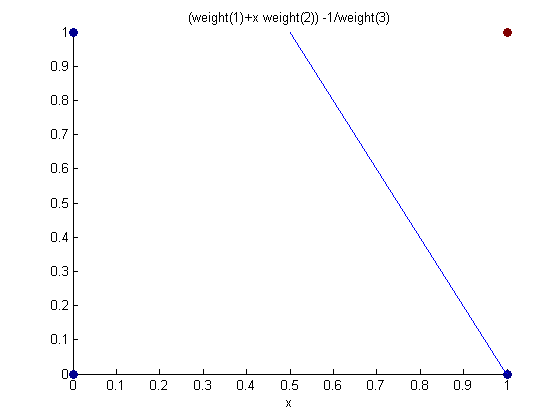
\includegraphics[scale=0.5]{img/and_correct}
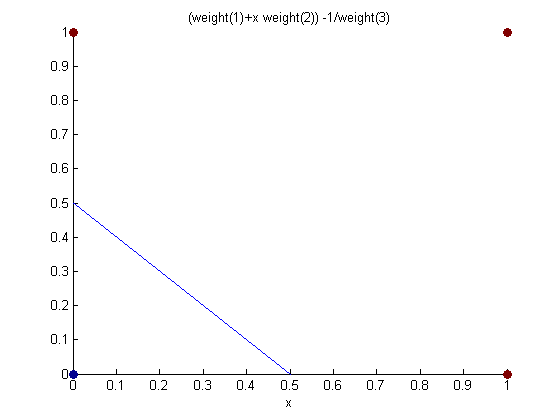
\includegraphics[scale=0.5]{img/or_correct}


The following images show a dataset of 200 entries with the points classified differently. The image on the left has the points classified in a way so that they're linearly separable and our algorithm performs ideally, while the points in the image on the right are scattered in a way that they can't be distinquished by a line. The drawn line separates the points in a way that 142 of them are classified correctly.


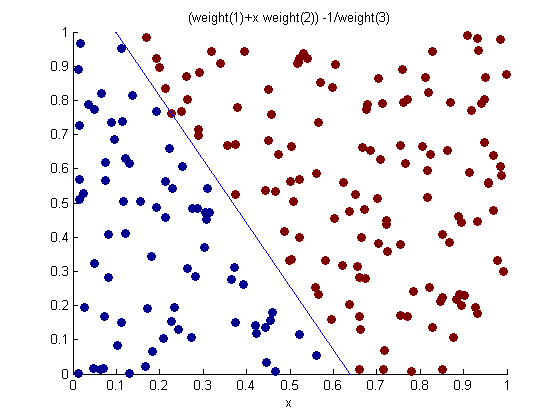
\includegraphics[scale=0.5]{img/200_of_200_correct}
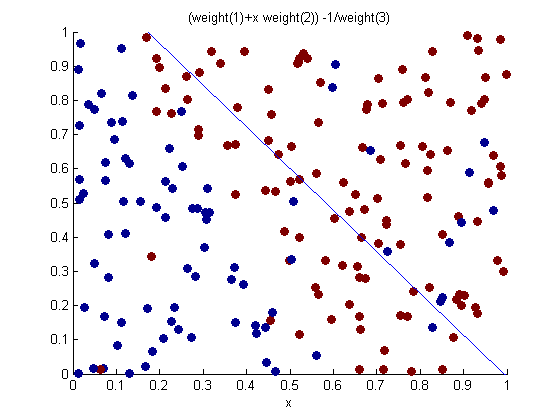
\includegraphics[scale=0.5]{img/142_of_200_correct}

\section{Practical Application}

Hier erklären wir was wir jetzt vorhaben, wie die Trainingssets bzw Eingangsdaten aussehen und was dann hoffentlich passieren wird / was wir versuchen herauszufinden

Prepare a scientific report comparing the performance of the three classification
algorithms on your chosen dataset on the two problems describ d above. In-
clude graphs showing the different classification rates. Discuss and interpret the
results. Can you think of good reasons for the different results produced by the
different classifers? Which combination of the 10 rejected infrared light wave-
lengths (column 1-10 at file strokefeatures.mat) leads to the best results?
Does using fewer features improve the p erformance? What is a good way to
chose the best features to keep? Is you classifer good enough to be used in real
life? Your discussion should be precise and scientific. 

\subsection{Perceptron Stuff}

Wie hat das ganze mit Perceptron funktioniert. Verwendete Datasets, Eingaben, Ausgaben, Analyse der Ausgaben: wie richtig ist das ganze, funktioniert es in allen Fällen oder in manchen nicht? Wo (mit welchen Sets / Eingaben) funktioniert es besser, wo schlechter?

\subsection{kNN Stuff}

Same for kNN

\subsection{Mahalanobis stuff}

same for mahalanobis

\section{Comparison Perceptron / Pattern Recognition}

Wie haben die Methoden im Vergleich zueinander abgeschnitten? Wo lagen bei ihnen SChwächen und Stärken? Genauigkeit? 


\section{Extra-Aufgabe?}

\section{Conclusion}

Hier kommt dann noch ne kurze Zusammenfasung rein.



\end{document}
